\documentclass{article}
\usepackage[utf8]{inputenc}
\usepackage{xcolor}
\usepackage[margin=1in]{geometry}
\usepackage{hyperref}
\usepackage{graphicx}
\usepackage{booktabs}

\usepackage[backend=biber,style=ieee,sorting=none]{biblatex}

\addbibresource{refs.bib}

% command for red text 'todo' items
\newcommand\todo[1]{\textcolor{red}{TODO: #1}}

\title{CS766 -- Mid-Term Report \\ Super Resolution Image Enhancement}
\author{Asher Elmquist (\texttt{amelmquist@wisc.edu}) \\
Eric Brandt (\texttt{elbrandt@wisc.edu})
}
\date{Due: April 1, 2020}

\begin{document}

\maketitle

\section{Overview}

The high-level goal of our project is explore image super-resolution and understand how creating higher resolution or higher quality pictures can assist in downstream tasks such as object recognition or image segmentation. The original proposal (see Appendix \ref{app:proposal}) contains detailed information about the relevance of this topic as well as our intended methods of investigation.  This report serves the following purposes:
\begin{itemize}
    \item Report on progress and results achieved thus far
    \item Explain unexpected challenges and difficulties that have been encountered
    \item Define remaining tasks and timelines
\end{itemize}

\section{Progress}

\subsection{Training Data}
The training, validation, and test data for our project consists of images from the OpenImages V5 Dataset \cite{OpenImages}\footnote{The V6 dataset was released in February 2020. We began our project before that release, and therefore our work is based on the V5 dataset}.  The full data set consists of an astonishing 9 million images with a combination of human-verified and machine-generated labels. For our training, we decided to focus on training using a subset of these images. After reviewing the labels in the entire dataset, we chose four distinct labels on which to focus: `Building,' `Dog,' `Flower,' and `Food.' Our hope in narrowing down the scope of image content, we might facilitate future intra- and cross-label inference testing.

After deciding on the appropriate images to use, the acquisition of a data set was broken down into 3 phases: image retrieval, training image preparation, and comparison image preparation.

\subsubsection{Image Retrieval}
Simply managing the process of acquiring the images was a formidable task. For example, the \texttt{.csv} file containing the image identifiers, their corresponding label identifiers, and their web locations is a 3.2 GB file, which itself had to be parsed and searched for images containing the labels of interest. A python script (\href{https://github.com/elbrandt/CS766_Project/blob/master/dataset/Retriever/Retriever.py}{Retriever.py}) was written to perform this task. Because we wanted to focus on large, high resolution images, we used the file size (contained as a field in the \texttt{.csv} file) as a heuristic, and only downloaded images that a) had one of our labels, and b) had a file size greater than 5MB. The script was allowed to run for approximately 12 hours, downloading copyright-free and royalty-free images meeting these criteria from the web.

\subsubsection{Training Image Preparation}
Once a sufficient number of candidate images having each label were downloaded, we prepared the images using a second Python script (\href{https://github.com/elbrandt/CS766_Project/blob/master/dataset/Retriever/Resizer.py}{Resizer.py}). Using OpenCV \cite{opencv_library}, this script opened each image and performed the following operations:
\begin{enumerate}
    \item If the image had a resolution under 2048x2048, the image was discarded from the training set. We are only interested in high resolution images.
    \item The image was center-cropped to 2048x2048, to match the input dimensions of our training network. This full-resolution crop was saved.
    \item The image was then incrementally downsampled using bilinear interpolation by factors of 2, saving at each resolution. Each image was saved at square resolutions of 2048, 1024, 512, 256, 128, and 64. 
\end{enumerate}
We note that at the lower resolutions (e.g. 64x64), the image quality was significantly higher if the scaling was performed in `steps,' visiting each intermediate power of two enroute to the final resolution. Image quality was much worse if we rescaled directly from the high resolution to the low resolution. Therefore, we settled on the former approach to build our training images.

After this phase, our training data set consisted of the images shown in Table \ref{tab:img-count}.
\begin{table}[h]
\centering
\begin{tabular}{@{}lc@{}}
\toprule
Label    & \multicolumn{1}{l}{\# of Images} \\ \midrule
Building & 24,530                           \\
Food     & 17,855                           \\
Dog      & 10,736                           \\
Flower   & 24,100                          
\end{tabular}
\caption{Image quantity for each label in our data set}
\label{tab:img-count}
\end{table}

\subsubsection{Comparison Image Preparation}
The above steps produced ample training data. However, to compare our super-resolution method with `traditional' upscaling methods, we also generated a comparison data set. To do this, a third Python script (\href{https://github.com/elbrandt/CS766_Project/blob/master/dataset/Retriever/Upsampler.py}{Upsampler.py}) was written. This script takes as input a `starting' and `ending' resolution. It then traverses the local data set, and upscales all images that are saved at the `starting' resolution using bilinear interpolation to the `ending' resolution.  The output of this process gives us a point of comparison for our method versus the most widely used traditional method for increasing image resolution.

\subsection{Network Architecture and Training Procedure}

Based on existing work in image super-resolution, we implemented a convolutional network that utilizes progressive upsampling to produce an image at the target resolution. While other upscaling methods exist, progressive upscaling has been shown to avoid the issues of pre or post-upscaling \cite{wang2018fully,lai2017deep}. Pixel shuffle is used as the upsampling layer as this avoids the some checkerboarding artifacts produced through transposed convolution \cite{aitken2017checkerboard}. The full implemented architecture is shown in fig. \ref{fig:nn_arch}. The implementation, written using PyTorch \cite{NEURIPS2019_9015}, includes input and output convolution layers with a ResNet \cite{he2016deep} and PixelShuffle block for each doubling of resolution. Optionally, noise can be added at each upsampled resolution to assist in detail creation \cite{karras2019style}. 

\begin{figure}[h!]
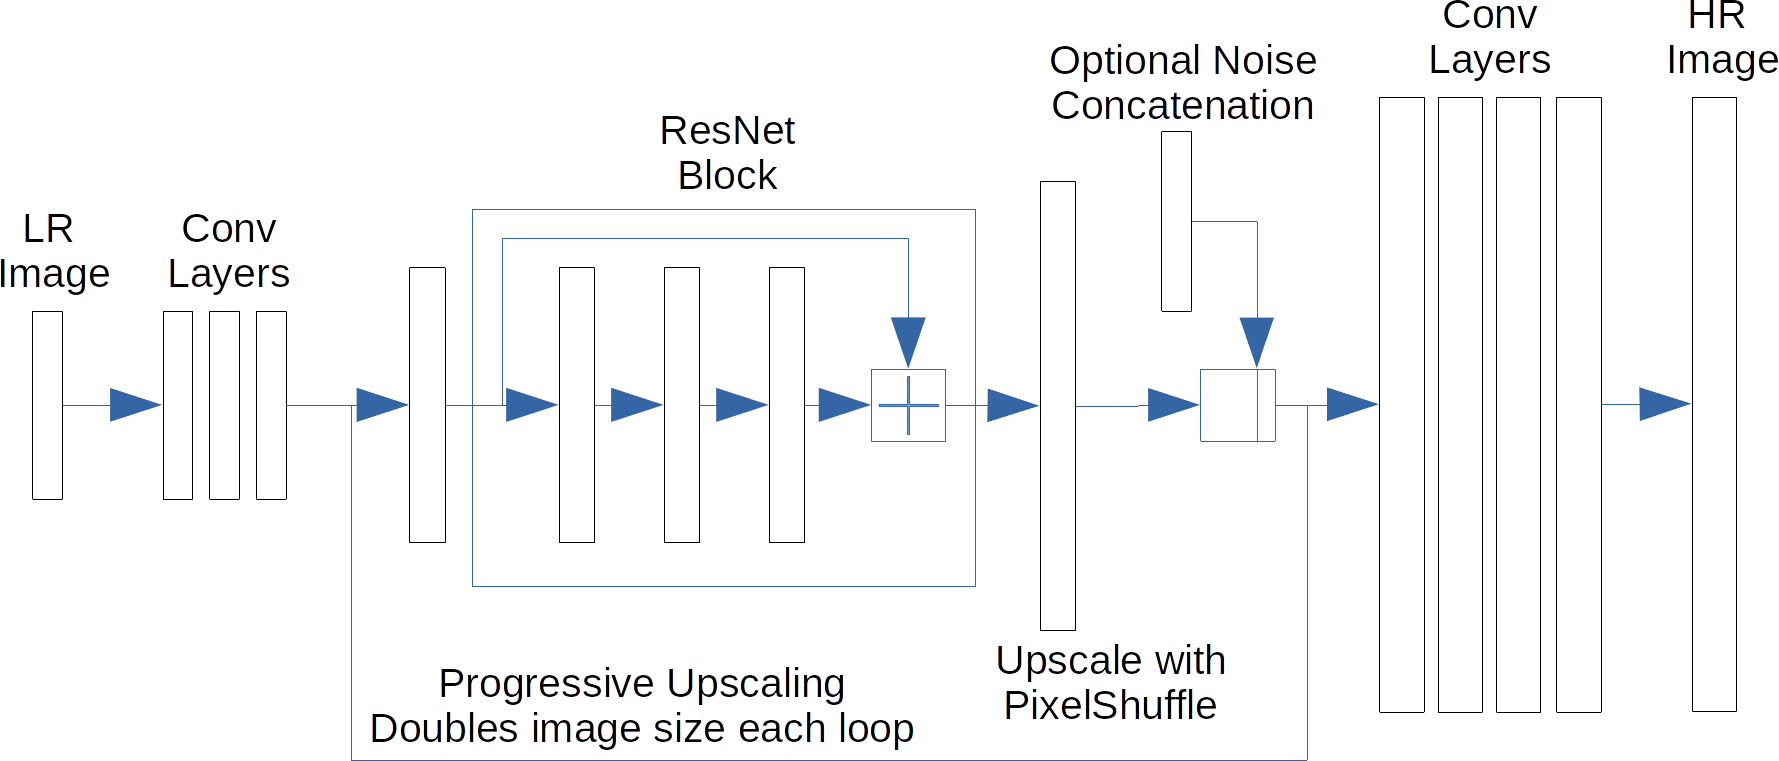
\includegraphics[width=\textwidth]{midterm_results/network_arch.png}
\caption{\textit{Flowchart illustrating the neural network architecture used for super-resolution. The network is based on best practices from existing image super resolution and image translation networks.}} \label{fig:nn_arch}
\end{figure}

The loss used for generating the priliminary results shown in this report uses mean squared error (MSE) loss between the generated image and the target image. While this reduces the the pixel error, it often results in a lack of high frequency detail. To mitigate this issue, we will introduce a second term in the loss function to additionally minimize the content loss follow \cite{johnson2016perceptual}.

For training the network, we use the data sets previously discussed. For the preliminary results, we used 24000 images from our building data set. Since we generated intermediate results, we used those to train the network progressively. That is we trained the network to learn 64x64 to 128x128 super resolution. Once the training had converged, we retained the trained weights and introduced another upscaling block. The pretrained layers continue to be trained for higher resolutions, but the progressive growing strategy has been shown to reduce training times and improve convergence \cite{lai2017deep,karras2017progressive}. 



\subsection{Website and Code Repository Status}
The project code as described above resides in the Github repository located at

\texttt{\href{https://github.com/elbrandt/CS766_Project}{https://github.com/elbrandt/CS766\_Project}}.

\noindent The project website has been updated to reflect current progress and is located at

\texttt{\href{https://elbrandt.github.io/CS766_Project/}{https://elbrandt.github.io/CS766\_Project/}}.

\section{Inference Results of Initial Training}
Figures \ref{fig:food_examples} and \ref{fig:building_examples} each contain two example images from our food and building data sets respectively. Each began as a high resolution image (2048x2048). It was progressively downsampled to 64x64, shown in the left-most column. The low-res image was then used as input to the trained Super-resolution CNN model to be up-sampled to 512x512. The output appears in the second column. The third column contains the results of a bilinear interpolation upsampling of the low-res image for comparison. Finally, the right column contains the ground-truth image. 

\begin{figure}[h!]
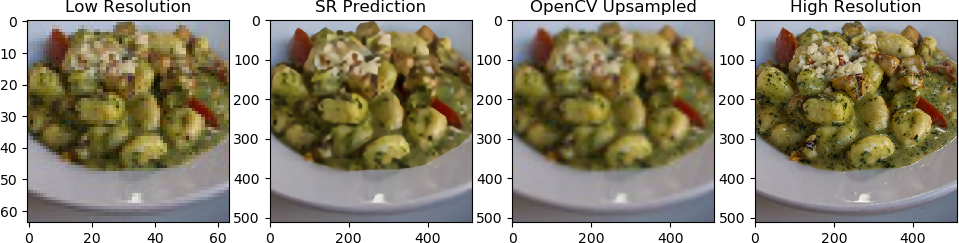
\includegraphics[width=\textwidth]{midterm_results/test_img_0.png}
\par\medskip
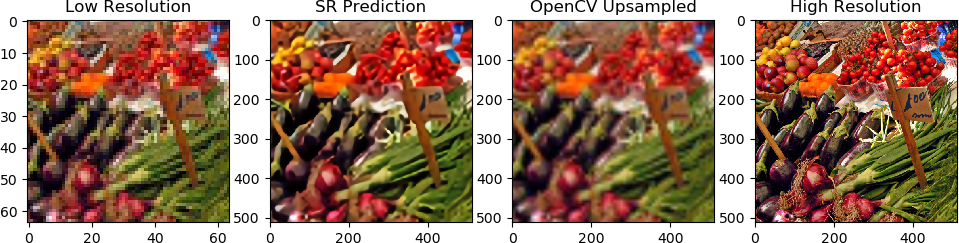
\includegraphics[width=\textwidth]{midterm_results/test_img_1.png}
\caption{\textit{Two example images from the food dataset (model trained on buildings). Left-to-right: Low-res input, Super-resolution prediction, bilinear upsampling, original high-res image.}} \label{fig:food_examples}
\end{figure}

\begin{figure}[h!]
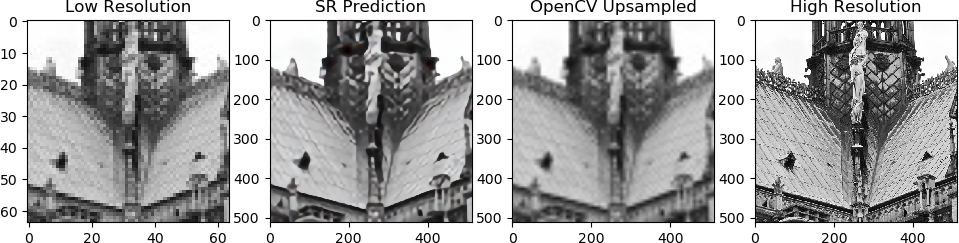
\includegraphics[width=\textwidth]{midterm_results/test_img_6.png}
\par\medskip
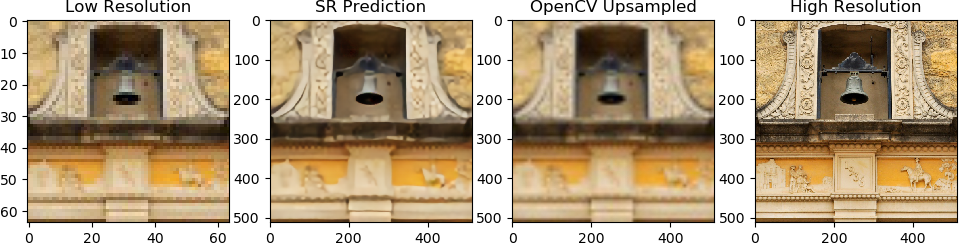
\includegraphics[width=\textwidth]{midterm_results/test_img_11.png}
\caption{\textit{Two example images from the buildings dataset on which the model was trained. Left-to-right: Low-res input, Super-resolution prediction, bilinear upsampling, original high-res image.}} \label{fig:building_examples}
\end{figure}

\section{Challenges / Difficulties}
\subsection{Data Set Generation}
Finding a copyright-free source of high quality, accurately labeled images turned out to be more difficult than we originally thought. Most online data sets available online for purposes of deep learning training typically suffer from either a) being low resolution, b) being high resolution, but not being labeled, or c) being extremely narrow in scope. Image sets of high resolution images that are already accurately labeled are typically copyright, or the terms of use expressly forbid high-volume downloads for the purposes of machine learning.  

The data set we found and used does satisfy both our requirements (high resolution, and labeled). However, the data set still suffers from two issues: 
\begin{enumerate}
    \item The data set is not uniformly high resolution. Images of all resolutions are mixed in, and the resolution is not known until the image has been downloaded. 
    \item While the labeling on the images is generally accurate, for many of the images we downloaded, the label is not unique nor the primary subject of the image. For example, images labeled `food' would ideally all be images that one might see on a menu at a restaurant: a plate of food and nothing else. However, our data set `food' images include such things as `raw materials of food' (e.g. fields of corn), pictures of restaurant fa\c{c}ades, scenes of people eating at a party, and of course, some pictures specifically featuring prepared food as the primary and only subject of the photograph.
\end{enumerate}
The first issue can easily be addressed by simply ignoring images below a certain resolution. The second issue is much harder - in that it typically would require manual inspection of each image to determine if an image met our own subjective criteria of what we had in mind when we chose the label `food.' This is intractable for the quantity of images we are using.

This limitation of 'label-subject quality' in our data set may have significant impact on the ability to evaluate the impact of `cross-label' versus `same-label' inferences. For example, we may not be able to effectively evaluate whether a CNN trained on images of `buildings' does better or worse at inferencing other `building' images than it does at inferencing `food' images.

\subsection{Trained Model Inference}
While our results thus far appear to be closer to the high resolution image than bilinear interpolation, our results do have some small artifacts. Primarily, our results lack the high-frequency detail seen in the HR image. This is in line with previous state-of-the-art SR  networks. The proposed addition of content loss should improve this issue.

Another issue which we can easily accommodate in our project, but may prove difficult in a real application, is the resolution and aspect ratio dependence on the input images. We have chosen to train exclusively on square images whose resolution is a power of 2, because this works nicely with our CNN structure. However, in the real world, camera sensors are rarely at this aspect ratio nor are a power-of-two resolution. It is unclear from existing literature how to generalize a trained network to perform on images of arbitrary input resolution.

\section{Remaining Tasks}
Based on the initial project proposal and the adjustments made as a result of our preliminary results, the remaining tasks are as follows,
\begin{itemize}
    \item improve the training by augmenting the loss function to include content loss based on VGG
    \item perform domain specific super-resolution study to quanitify effect of image content on super-resolution
    \item setup image segmentation for SR benchmark
\end{itemize}



\subsection{Re-alignment of Goals}
For the remainder of the project, we have realigned our goals based on further research and understanding after implementation of initial networks. The original goal of understanding domain specific super-resolution will be maintained, but may not be as significant based on the data set challenges discussed earlier in the report. Additionally, we will shift from using object detection for understanding if we can predict sub-pixel object positions to using image segmentation to understand if super-resolution can improve sub-pixel prediction of object boundaries. We will use a pre-trained segmentation network to evaluate and understand these results.

The readjusted goals are now as follows,

\begin{enumerate}
    \item Implement super-resolution network based on current research in the field
    \item Study domain-specific super resolution to understand the effect of image attributes on SR
    \item Perform image-segmentation to understand the improvement SR can give for predicting sub-pixel object boundaries
\end{enumerate}

\subsection{Performance Metrics}

The results shown in this progress report are preliminary and are for visual inspection only with no quantitative performance metrics yet implemented. For the final report and the remainder of the project, we will use two primary metrics. The first metric is a scoring measure used for the 2017 NTIRE super-resolution challenge, found here: \url{https://data.vision.ee.ethz.ch/cvl/DIV2K/}. The second metric will be based on image segmentation. Segmentation, based on pre-trained models, will be used to evaluate the accuracy of the SR results in predicting sub-pixel object boundaries. We will use the high resolution segmentation results as ground truth. In addition to providing an accuracy metric, this will allow us to understand and evaluate SR as a method for the application of higher resolution segmentation.

\subsection{Revised Timeline}
Based on the re-alignment of goals, our timeline going forward is as follows:

\begin{itemize}
    \item \textbf{April 1st:} Project Mid-Term Report Due.
    \item \textbf{April 8th:} Finish revision and tweaking of models, begin large-dataset training. Begin evaluating and preparing performance metric test.
    \item \textbf{April 15th:} Begin evaluating performance. Begin working with image segmentation models.
    \item \textbf{April 22nd:} Compile final tests and results data. Begin work on video presentation.
    \item \textbf{April 29th:} Assemble project report, web page, and video presentation.
    \item \textbf{May 4th:} Project web page \& video presentation due.
\end{itemize}

\appendix

\section{Original Proposal}\label{app:proposal}

The original proposal, as submitted, is included here for reference.

\subsection{Project Overview}
The purpose of this project is to explore image super-resolution and understand how creating higher resolution or higher quality pictures can assist in downstream tasks such as object recognition or image segmentation. To understand the effect of super-resolution, we propose implementing a convolutional neural network for super-resolution based on the current state of the art. Beyond recreation of a current algorithm, we will study the general nature of the trained model, and explore the application of super-resolution in object detection accuracy and precision. This document covers the relevance of the project, a brief outline of the state of the art, a detailed description of the project plan, and a timeline that we plan to follow in order to accomplish the outlined tasks. 


\subsection{Project Relevance}
Generating super-resolution images from low resolution images has been used in medical imaging \cite{Pham2019, Georgescu2020}, astronomy imaging \cite{zhang2019} and security imaging \cite{yang2019deep}. Where small or blurry objects need to be identified, a higher resolution image may increase the performance of existing object recognition algorithms. If super-resolution techniques deliver on their promises efficiently, we can transparently substitute lower resolution or more highly compressed images for costly high resolution images. Image storage, network transmission and video encoding/decoding  are several examples of the utility of this. Super-resolution is an interesting task in and of itself, but we propose this project as a way to better understand and explore the potential for super-resolution networks to occupy one step in a pipeline for object detection or semantic segmentation tasks. The ability to locate objects potentially with sub-pixel precision in an image has interesting future applications for photogrammetry and metrology. To this end, our proposal centers on the implementation and application of super-resolution.


\subsection{State of the Art}
A recent and comprehensive overview of state of the art super-resolution algorithms and network structures can be found in \cite{yang2019deep}. A short discussion of key points as well as important notes will be given here as they relate to the project proposal. This discussion will cover generative adversarial networks (GANs) versus supervised learning for super resolution as well as a well-studied network structure that has been shown to work well in image enhancement architectures: ResNet \cite{he2016deep}.

The problem of super-resolution (SR) is in the non-uniqueness of a high-resolution (HR) image generated from a lower-resolution (LR) image. For any LR there are multiple plausible HR that would be faithfully represented by the LR. One way to generate data for SR is to down sample an HR image. Unfortunately, generating training samples from down sampling can lead to small artifacts in the network when trained to directly undo the down sampling algorithm \cite{yang2019deep}. One way of circumventing this is to use an unsupervised learning approach so as not to unwittingly compute a mapping from input-output samples, but instead to compute a mapping from a distribution of inputs to a distribution of outputs. Generative adversarial networks accomplish exactly this and have been shown to work well for SR \cite{ledig2017photo}. While GANs would improve SR on real-world low-resolution images, we can explore SR in a more efficient manner when we have more control of the datasets and training as is the case with the supervised approach. State of the art results are shown from a supervised method in \cite{lim2017enhanced}.

In super-resolution, the network architecture plays an important role in the accuracy and efficiency of the network. Many image processing network architectures (including SR) are built on a well-studied convolutional network called ResNet. This network uses a recursive structure to learn small changes in the image. The network is made up of residual blocks with a fraction of the input added directly to the output of a later  block. These connections are known as skip connections and are a fundamental component of the ResNet architecture \cite{he2016deep} to reduce the complexity of the loss surface and reduce convergence to local minima. These residual blocks, along with up-scaling via deconvolution form the basis of many SR network architectures \cite{yang2019deep} and are detailed in the implementation given in \cite{lim2017enhanced}.

\subsection{Project Plan}
The project will be split into four sections that will allow exploration beyond the state of the art. The first part of the project will be to recreate state of the art super-resolution results using machine learning. In itself this is a difficult task, but there is significant room to explore beyond what has been discussed in the previous section. To go further, we propose studying the generalization of the trained network by training and testing across different image domains. That is, we will train on a set of images, say buildings, and then evaluate the network on an animal image data set. In addition, we propose applying state-of-the-art, off-the-shelf object detection networks such as YOLO-V3 \cite{redmon2018yolov3} and SSD \cite{liu2016ssd} to understand if object recognition can be improved using super-resolution. Time-permitting, we will then extend to understand if other image improvement could help with object detection such as denoising or sharpening. Since similar networks for super-resolution can be modified for general image enhancement, this is a natural continuation of the project. Finally, we hope to pay attention to the time required to perform SR on images of particular sizes to evaluate the efficacy of real-time SR for live-acquisition applications on either general-purpose or dedicated hardware. Further details and data plans are laid out in the following sections.


\subsubsection{Implement and Train Super-Resolution Network}
Following the state of the art implementations, we will use a residual CNN as it has been shown to reduce error propagated across layers when given sufficient skip connections. To limit training time, we will avoid using generative adversarial networks. This will result in requiring the network to be trained through supervised learning, meaning we will require input and output image pairs. We do not foresee this being an issue as we can generate a dataset from a single set of high resolution images. This will also give us flexibility in the resolutions we choose to understand the extent to which resolution can be increased without unintended artifacts. For verification, our super-resolution can be compared against ground truth (original image) and bicubic or bilinear interpolation of the downsampled/corrupted image. We can also qualitatively compare our results to state-of-the-art results from the papers discussed previously.


\subsubsection{Run Domain Transfer Study}
We propose studying the general nature of our network by having three distinct datasets. These may be, for example, buildings, cars/roadways, and animals, each of which have a large corpora of readily available data. We will then hold out one dataset during training to use during testing to see if there are domain specific artifacts that appear on images with significant content differences. We will apply this holdout to each subset in turn to understand the full effects.


\subsubsection{Apply Object Detection Networks}
To understand if super-resolution improves object detection, YOLO-V3 and SSD will be used with pretrained weights. These networks have been shown to give state-of-the-art object detection accuracy. The accuracy of the pretrained networks will be run on the lower resolution images to generate a baseline accuracy for comparison. The networks will then be run on the higher resolution (cropped when necessary to create one-to-one comparison) to understand if super-resolution improves detection rate, position-precision, or class confidence. Multiple data sets will also allow us to understand if there is significant difference when detecting difference object classes.


\subsubsection{Further Extend To General Image Enhancements}
If time permits, we can extend this project to look at other image enhancements for improving object detection. Since the residual CNNs have the same architecture as general image processing networks, the network proposed can be adjusted and trained to denoise, or sharpen images at the lower resolution. We would then perform the same studies discussed above on the resulting denoised or sharpened images.


\subsection{Web Page}
A project web page that will track progress and summarize results has been set up at 
\begin{itemize}
    \item \url{https://elbrandt.github.io/CS766_Project/}.
\end{itemize}

\noindent All materials related to the project will be tracked in the GitHub repository located at 

\begin{itemize}
    \item \url{https://github.com/elbrandt/CS766_Project}.
\end{itemize}


\subsection{Timeline}
In order to meet the class deadlines and adhere to the project plan, the following timeline is proposed.

\begin{itemize}
    \item \textbf{February 14th:} Project Proposal Due 
    \item \textbf{March 13th:} Complete Super-Resolution Implementation
    \item \textbf{March 20th:} Complete Domain Transfer Study
    \item \textbf{March 25th:} Project Mid-Term Report due \textit{Possible re-alignment of goals based on progress thus far}
    \item \textbf{April 3rd:} Complete Object Detection Study
    \item \textbf{April 17th:} Complete Additional Image Enhancement Study
    \item \textbf{April 27-May 1st:} Project Presentations
    \item \textbf{May 4th:} Project Webpage Due
\end{itemize}


\printbibliography
\end{document}


